This section delves into the process of learning attack frequencies from \cmt{input dataset}. We assume attacks occur within specific timeframes, as illustrated in \fig{attacks}. The Mean Time Between Attacks (MTBA) is extracted from the dataset using established algorithms like the Broyden–Fletcher–Goldfarb–Shanno (L-BFGS-B) algorithm described in \cite{liu1989limited} and the Nelder-Mead algorithm \cite{nelder1965simplex}. \cmt{Section~\ref{sec:rw} will discuss additional algorithms inspired by natural behaviors \cite{Genghis2023, Ezugwu2022, Jeffrey2022, Agushaka2023, Mojtaba2024, DETDO2023} that can be employed for this purpose.}



\begin{figure}[h]
\noindent
     \centering
		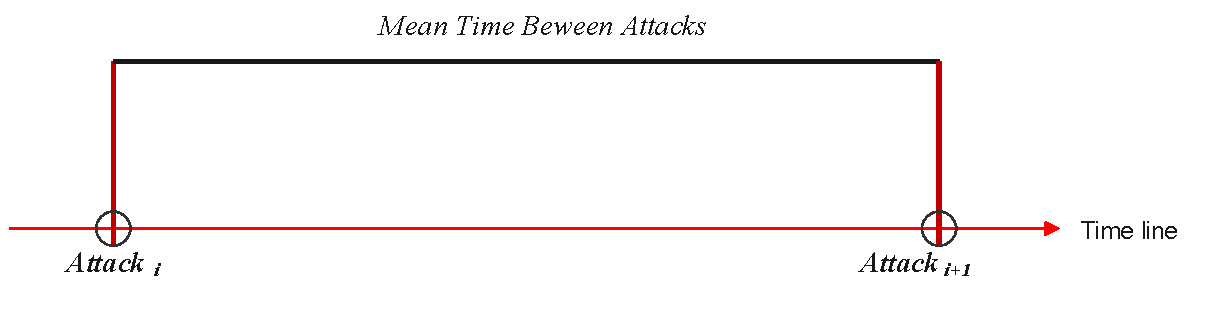
\includegraphics[width=300pt, height =100pt]{timeline.pdf}
		\caption{Mean Time Between Attacks}
	\label{attacks}
\end{figure}



%The L-BFGS algorithm is widely employed for optimizing problems involving large datasets. On the other hand, the Nelder-Mead algorithm, also known as the downhill simplex method, constructs a geometric shape in the parameter space to search for the optimal solution efficiently. 

The classical approach for calculating the mean time involves considering the initial attack detected along with its successors, divided by the total number of attacks in the dataset. Formally, for a dataset consisting of \emath{n} features: \emath{f_{1},\ldots, f_{n} \in F}  where each feature is associated with its domain \emath{ Dom: F \rightarrow \mathbb{D}}. \emath{\mathbb{T}} is the time domain for attack feature occurrence. We are able to implement the Algorithm \ref{algo:attacks}. The algorithm is a simple exploration of the dataset where two attacks are collected \emath{a_{1}} and \emath{a_{2}}, where \emath{a_{2}} is the successor of \emath{a_{1}}. When an attack is detected, its successor is determined and the difference is stored in the stack. Subsequently, the mean time between attacks is calculated once the successor is empty. For handling large datasets, we utilize both the L-BFGS and Nelder-Mead algorithms. The Python source code for this implementation can be found in the Artefacts section \ref{sub:artefact}.

\RestyleAlgo{ruled}

%% This is needed if you want to add comments in
%% your algorithm with \Comment
\SetKwComment{Comment}{\gtext{/*} }{ \gtext{*/}}
\begin{algorithm}[H]
\label{algo:attacks}
\caption{Mean Time Between Attacks Computation. }
%\caption{An algorithm with caption}\label{alg:two}
\KwData{Feature \emath{f_{i}.}}
\KwResult{p as attack frequency.}
$Stack \gets Empty$ \Comment*[r]{\gtext{A stack of meantime of attacks.}}
$a_{1} \in \mathbb{T}$ \Comment*[r]{\gtext{initial attacks.}}
$a_{2} \in \mathbb{T}$ \Comment*[r]{\gtext{sucessor of the attack.}}
 
\For{ line \emath{\in} dataset }{ 
     \If{attack \emath{\in} line}    {
            $a_{1} = extractTimefrom feature(f_{i}, attack)$ \Comment*[r]{\gtext{Extract the first attack.}}
            
            $a_{2} = extractNextAttackTimefromfeature(f_{i}, attack)$\Comment*[r]{\gtext{Extract the successor of the first attack.}}
            
            $Stack.append(|a_{2}-a_{1}|)$\Comment*[r]{\gtext{Store the time differences}}
        }
        
     \If{$a_{2}$ is $Empty$}    {
            $satisfy \gets false$;

            $p \gets meanTime(Stack)$ \Comment*[r]{\gtext{Store the calculated mean time as the probability of an attack occurring.}}
        }

             

}
\end{algorithm}
